\chapter{Spectral Method} \label{chap:spectral-method}
In Chap.~\ref{chap:polynomial-eigenvalue-problem}, we explored the analytical solutions, including eigenvalues and eigenfunctions, to Eq.~(\ref{eq:constant-v-problem}), a special case of a more general polynomial eigenvalue problem Eq.~(\ref{eq:polynomial-eigenvalue-problem}). As we can see, it is nearly impossible to solve Eq.~(\ref{eq:polynomial-eigenvalue-problem}) analytically. Hence, we need numerical methods to investigate the instability of plasma flow with spatial varying velocity profile. Spectral methods is a suitable tool for our problem.

Spectral method is an important tool for solving problems related to partial differential equations. It can provide superior accuracy compare to other local methods such as finite difference \cite{shen_tang_etal_spectral_2011}. In this thesis, we are going to solve a polynomial eigenvalue problem, i.e. Eq.~(\ref{eq:polynomial-eigenvalue-problem}) together with specific boundary conditions.

Suppose the velocity perturbation $\tilde{v}$ can be approximated by some orthogonal basis functions $\{u_k(z)\}_{k=1}^{\infty}$ on $-1\leq z\leq 1$,
\begin{equation}
	\tilde{v} = \sum_{k=0}^{N} c_ku_k(z),
\end{equation}
where $c_k$ are coefficients to be determined. There are different choices for $u_k(z)$ including but not limited to \cite{shen_tang_etal_spectral_2011},
\begin{itemize}
	\item $u_k(z)=T_k(z)$ (Chebyshev spectral method)
	\item $u_k(z)=L_k(z)$ (Legendre spectral method)
	\item $u_k(z)=H_k(z)$ (Hermite spectral method)
\end{itemize}
where $T_k$, $L_k$ and $H_k$ are Chebyshev, Legendre, and Hermite polynomials of degree $k$.

Using the above approximation in Eq.~(\ref{eq:polynomial-eigenvalue-problem}), and take the inner product with some other test functions $\{\psi_k(z)\}$ on $[-1,1]$, the left-hand side of Eq.~(\ref{eq:polynomial-eigenvalue-problem}) becomes a matrix equation,
\begin{equation}
	(\omega^2\mathbf{1} + \omega\mathbf{M} + \mathbf{N})\mathbf{c} = \mathbf{0},
	\label{eq:pep-matrix-equation}
\end{equation}
where $\mathbf{c} = [c_0, \cdots, c_N]^T$ is a vector of coefficients, and
\begin{align}
	M_{jk} & = 2i\int_{-1}^{1}dz \; \psi_{j}\left(v_0\pdv{}{z} +\pdv{v_0}{z} \right)u_{k}
	\label{eq:operator-matrix-M}                                                          \\
	N_{jk} & = \int_{-1}^{1}dz \; \psi_{j} \left[(1-v_0^2)\pdv[2]{}{z}
		-\left(3v_0 + \frac{1}{v_0}\right)\pdv{v_0}{z}\pdv{}{z}
		- \left(1-\frac{1}{v_0^2}\right)\left(\pdv{v_0}{z}\right)^2
		- \left(v_0+\frac{1}{v_0}\right)\pdv[2]{v_0}{z}\right] u_{k}
	\label{eq:operator-matrix-N}
\end{align}

Depending on the choice of the test function, spectral method can be further classified \cite{shen_tang_etal_spectral_2011},
\begin{itemize}
	\item Galerkin: The test functions are the same as the trial ones, i.e. $\psi_k=u_k$.
	\item Collocation:  The test functions $\{\psi_k\}$ are Lagrange basis polynomials such that $\psi_k(z_j)=\delta_{jk}$, where ${z_j}$ are preassigned collocation points.
\end{itemize}

To solve Eq.~(\ref{eq:pep-matrix-equation}), we simply augment the coefficient vector to $[\mathbf{c}, \omega\mathbf{c}]^T$. Then the matrix equation can be written as an algebraic eigenvalue problem,
\begin{equation} \label{eq:eigenvalue-problem}
	\mqty[ \mathbf{0} & \mathbf{1}\\ -\mathbf{N} & -\mathbf{M} ]\mqty[ \mathbf{c}\\ \omega\mathbf{c}] = \omega\mqty[ \mathbf{c}\\ \omega\mathbf{c}].
\end{equation}
We can apply standard eigenvalue problem solver to this question to obtain the eigenvalues $\omega$ and their corresponding eigenvectors $[\mathbf{c}, \omega\mathbf{c}]^T$. Therefore, the eigenfunctions $\tilde{v} = \sum_k c_ku_k(z)$ to the original problem can be recovered by extracting coefficients $\mathbf{c}$ from the eigenvectors.

\section{Spectral Collocation Method}
One of the methods we are going to use is called the Chebyshev collocation method.
Given a set of Chebyshev points, $\{z_j=\cos(j\pi/N)\}_{j=0}^{N}$, and let $\{h_j\}$ be the Lagrange basis polynomials associated with $\{z_j\}_{j=0}^{N}$, and define matrix $D_{kj} = h'_j(z_k)$. By setting $\tilde{v}(z) = \sum_{j=0}^{N}c_jh_j(z)$, we see that
\begin{align}
	\tilde{v}(z_k)   & = \sum_{j=0}^{N}\tilde{v}_jh_j(z_k) = c_k                         \\
	\tilde{v}'(z_k)  & = \sum_{j=0}^{N}\tilde{v}_jh'_j(z_k) = \sum_{j=0}^{N}D_{kj}c_j    \\
	\tilde{v}''(z_k) & = \sum_{j=0}^{N}\tilde{v}_jh''_j(z_k) = \sum_{j=0}^{N}D^2_{kj}c_j
\end{align}
We see that the coefficient vector $\mathbf{c}$ becomes a vector containing the values of $\tilde{v}$ evaluated at the collocation points, i.e. $\mathbf{c}=[v(z_0), \cdots, v(z_N)]^T$, and the matrix $D$ and $D^2$ act as the differential operators $\pdv{z}$ and $\pdv[2]{z}$, respectively. The matrix $D$ is called Chebyshev differentiation matrix since it acts as $\pdv{z}$ and evaluates at Chebyshev points.

\subsubsection*{Chebyshev Differentiation Matrix}
The Chebyshev differentiation matrix finds the derivative of the Lagrange interpolant of the given data points $(z_j,\tilde{v}(z_j))$ where $\{z_j = \cos(j\pi/N)\}_{j=0}^{N}$ are the Chebyshev points. Suppose $\mathbf{v} = [v(z_0), \cdots, v(z_N)]^T$, then the $N$-point, $D_N$, Chebyshev differentiation matrix gives $D_N\mathbf{v} \approx [v'(z_0),\cdots, v'(z_N)]^T$. Higher order differentiation can be achieved by taking powers of $D_N$. Thanks to \cite{trefethen_spectral_2000}, the construction of Chebyshev differentiation matrix is given in Fig.~\ref{fig:chebyshev-differentiation-matrix}.

If we instead use the equal-spaced points, $\{z_j=2j/N\}_{j=0}^{N}$, then the matrix defined by $D_{kj} = h'_j(x_k)$ will be the usual finite difference differentiation matrix. However, Chebyshev differentiation matrix has superior accuracy due to the wise choice of collocation points. On Fig.~\ref{fig:chebyshev-vs-fd} we see that the Chebyshev achieve higher accuracy.

\begin{figure} [htbp]
	\centering
	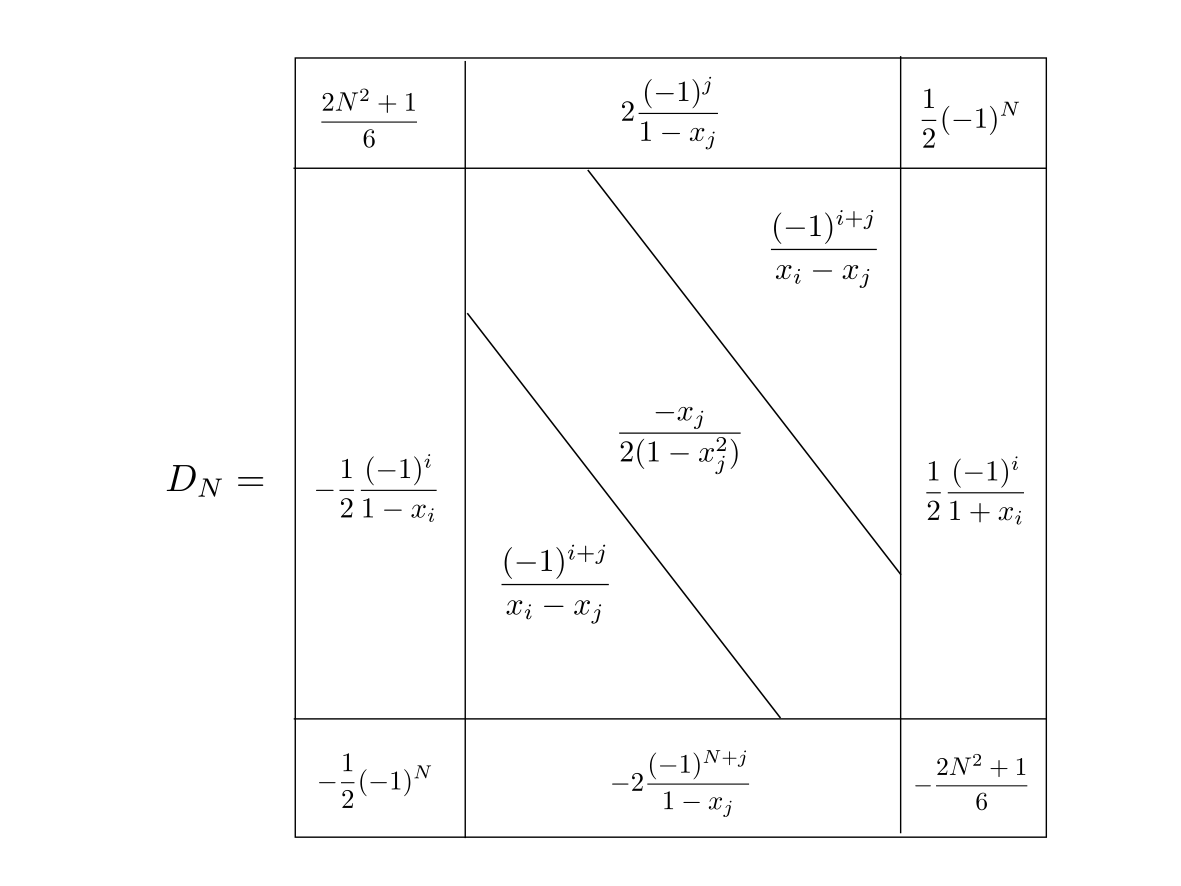
\includegraphics[width=\textwidth]{figures/chebyshev-differentiation-matrix.png}
	\caption{Construction of $N$-point Chebyshev differentiation matrix. The nodes $x_j = \cos(j\pi/N)$ are Chebyshev points. Adapted from \cite{trefethen_spectral_2000}.}
	\label{fig:chebyshev-differentiation-matrix}
\end{figure}

\begin{figure}
	\centering
	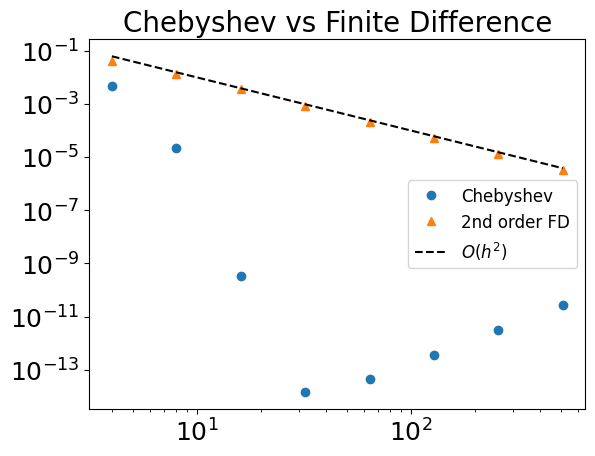
\includegraphics[width=0.7\textwidth]{figures/chebyshev-vs-fd.png}
	\caption{Comparison of accuracy between Chebyshev differentiation matrix and 2nd order finite difference differentiation matrix. Both methods are applied to compute the derivative of function $f(x)=\ln(2+\sin(x))$ on $[-1,1]$ using different resolutions, i.e. number of points $N$. We see that Chebyshev achieve higher accuracy using same amount of points.}
	\label{fig:chebyshev-vs-fd}
\end{figure}

\subsubsection*{Dirichlet Boundary}
To implement Dirichlet boundary condition, $\tilde{v}(\pm 1)=0$, to Eq.~(\ref{eq:pep-matrix-equation}), we only need to remove the first and last columns and rows of each matrix, $\mathbf{0,1,M}$, and $\mathbf{N}$. The reason is originated from the Chebyshev differentiation matrix, Fig.~\ref{fig:chebyshev-differentiation-dirichlet}. For a $(N+1)\times(N+1)$ Chebyshev differentiation matrix $D_N$, the first and last row has no effect since the first and last value of $\tilde{v}$ are $0$. We only need the interior of $D_N$ which is an $N\times N$ matrix. After solving Eq.~(\ref{eq:pep-matrix-equation}), we get the eigenvalues $\omega$ and their associated eigenfunctions evaluated at the interior collocation points $\mathbf{c} = [\tilde{v}_1,\cdots,\tilde{v}_{N-1}]^T$. We will need to prepend and append 0 to the eigenfunctions, $[0, \tilde{v}_1,\cdots\tilde{v}_{N-1}, 0]^T$. Listing.~\ref{code:spectral-collocation-dirichlet} has the pseudocode for solving Eq.~(\ref{eq:pep-matrix-equation}).

\begin{figure} [htpb]
	\centering
	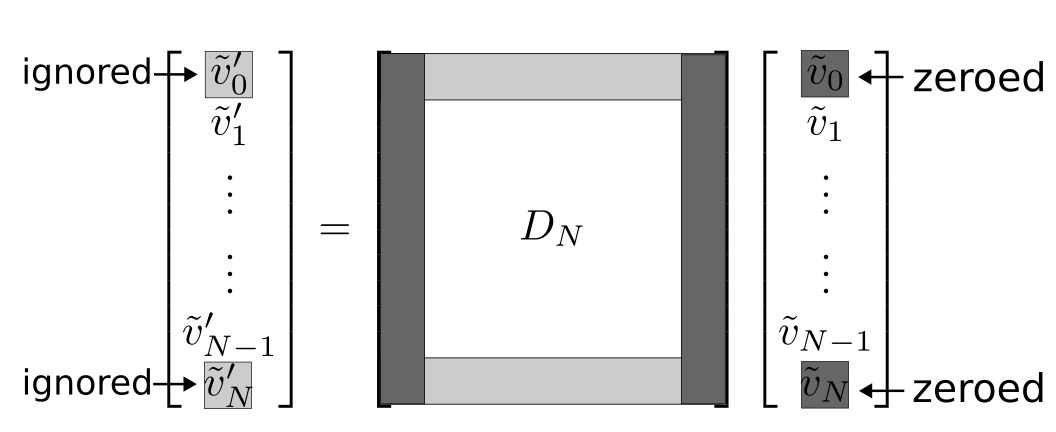
\includegraphics[width=0.7\textwidth]{figures/chebyshev-differentiation-dirichlet.png}
	\caption{Since the function $v$ is zero at $x_0$ and  $x_N$, the first and last columns has no effect and the same argument applies to first and last rows. Adapted from \cite{trefethen_spectral_2000}.}
	\label{fig:chebyshev-differentiation-dirichlet}
\end{figure}


\begin{lstlisting}[language=Python, float, floatplacement=H, caption={Pseudocode for solving polynomial eigenvalue problem using spectral collocation with Dirichlet boundary condition.}, label=code:spectral-collocation-dirichlet]
import numpy as np
# collocation points, differentiation matrices	
N = 101 # number of points
x, D1, D2 = Chebyshev(N) 
# solve polynomial eigenvalue problem
A11 = np.zeros_like(D1)
A12 = np.eye(*D1.shape)
A21 = -np.diag(1-v0**2)@D2 \
        + np.diag((3*v0 + 1/v0)*(D1@v0))@D1 \
        + np.diag((1-1/v0**2)*(D1@v0)**2) \
        + np.diag((v0+1/v0)*(D2@v0)) 
A22 = -2j*(np.diag(v0)@D1 + np.diag(D1@v0))
A = np.block([[A11[1:-1,1:-1], A12[1:-1,1:-1]],
              [A21[1:-1,1:-1], A22[1:-1,1:-1]]])
omega, V = np.linalg.eig(A)
# pad two ends of eigenfunctions by 0 (dirichlet boundary)
V = np.pad(V,((1,1),(0,0)))
\end{lstlisting}

\subsubsection*{Fixed-Open Boundary}
To implement fixed-open boundary condition, i.e. $\tilde{v}(-1)=\tilde{v}'(1)=0$. Notice that $\tilde{v}'(-1)$ can be expressed as,
\begin{equation}
	0 = \tilde{v}'(1) = \sum_{j=0}^{N}D_{ij}\tilde{v}_j,
\end{equation}
where $\tilde{v}_j=\tilde{v}(z_j)$ is the evaluation of $\tilde{v}$ at Chebyshev points $z_j=\cos(j\pi/N)$. By rearranging the terms, we get the expression of $\tilde{v}_0$ in terms of $\tilde{v}$ at other collocation points.
\begin{equation}
	\tilde{v}_0 = -\frac{1}{D_{00}}\sum_{j=1}^{N} D_{0j}\tilde{v}_j.
	\label{eq:expression-for-first-value}
\end{equation}
To incorporate this information into the differentiation matrix, we modify the expressions for evaluating the derivatives at point $x_1$,
\begin{align}
	\tilde{v}'_{1}  & = \sum_{j=0}^{N}D_{1j}\tilde{v}_j = \sum_{j=1}^{N}\left(D_{1j} - \frac{D_{10}}{D_{00}}D_{0j}\right)\tilde{v}_j        \\
	\tilde{v}''_{1} & = \sum_{j=0}^{N}D^2_{1j}\tilde{v}_j = \sum_{j=1}^{N}\left(D^2_{1j} - \frac{D^2_{10}}{D_{00}}D_{0j}\right)\tilde{v}_j.
\end{align}
This indicates the new differentiation matrices should be
\begin{align}
	D'_{ij} = \begin{cases}
		          D_{ij}, \quad                               & \text{if $i\neq 1$} \\
		          D_{1j} - \frac{D_{10}}{D_{00}}D_{0j}, \quad & \text{if $i=1$}
	          \end{cases} \\
	D'^2_{ij} = \begin{cases}
		            D^2_{ij}, \quad                                 & \text{if $i\neq 1$} \\
		            D^2_{1j} - \frac{D^2_{10}}{D_{00}}D_{0j}, \quad & \text{if $i=1$}
	            \end{cases}
\end{align}
After getting the eigenfunctions $\mathbf{c} = [\tilde{v}_1, \cdots, \tilde{v}_N]^T$, we need to prepend $\tilde{v}_0$ to $\mathbf{c}$ using Eq.~(\ref{eq:expression-for-first-value}). See Listing.~\ref{code:spectral-collocation-fixed-open} for pseudocode.


\begin{lstlisting}[language=Python, float, floatplacement=H, caption={Pseudocode for solving polynomial eigenvalue problem using spectral collocation with fixed-open boundary condition.}, label=code:spectral-collocation-fixed-open]
import numpy as np
# collocation points, differentiation matrices	
N = 101 # number of points
x, D1, D2 = Chebyshev(N)	
# modify second row to ensure v'(1)=0 
D1v = D1
D2v = D2
D1v[1,:] = D1[1,:] - D1[1,0]/D1[0,0]*D1[0,:]
D2v[1,:] = D2[1,:] - D2[1,0]/D1[0,0]*D1[0,:]
# only the differential operators acting on v needs to be modified
A11 = np.zeros_like(D1)
A12 = np.eye(*D1.shape)
A21 = -np.diag(1-v0**2)@D2v \
        + np.diag((3*v0 + 1/v0)*(D1@v0))@D1v \
        + np.diag((1-1/v0**2)*(D1@v0)**2) \
        + np.diag((v0+1/v0)*(D2@v0))
A22 = -2j*(np.diag(v0)@D1v + np.diag(D1@v0))
A = np.block([[A11[:-1,:-1], A12[:-1,:-1]],
              [A21[:-1,:-1], A22[:-1,:-1]]])
omega, V = np.linalg.eig(A)
# add v(1) to eigenfunctions
V = np.pad(V,((1,0),(0,0)))
for j in range(V.shape[1]):
    V[0,j] = -(D1[0,1:]@V[1:,j])/D1[0,0]
\end{lstlisting}


\section{Spectral Galerkin Method}
Another spectral method we used in the numerical experiments is the Legendre-Galerkin method. Meaning that the basis functions are chosen to be the compact combinations of Legendre polynomials \cite{shen_tang_etal_spectral_2011},
\begin{equation}
	u_k(z) = L_k(z) + a_kL_{k+1}(z) + b_kL_{k+2}(z),
\end{equation}
where the parameters $\{a_k,b_k\}$ are chosen to satisfy the boundary conditions. The test functions are the same as the basis functions.

Suppose the boundary conditions are
\[ a_{-}\tilde{v}(-1) + b_{-}\tilde{v}'(-1) = 0, a_{+}\tilde{v}(1) + b_{+}\tilde{v}'(1) = 0.  \]
Then the parameters $\{a_k,b_k\}$ can be worked out by simple linear algebra,
\begin{equation}
	\begin{aligned}
		a_k & = \frac{(2k+3)(a_{+}b_{-} + a_{-}b_{+})}{\text{DET}_k}                                              \\
		b_k & = \frac{-2a_{-}a_{+} + (k+1)^2(a_{+}b_{-} - a_{-}b_{+}) + b_{-}b_{+}k(k+1)^2(k+2)/2}{\text{DET}_k},
	\end{aligned}
\end{equation}
where $\text{DET}_k = 2a_{+}a_{-} + a_{-}b_{+}(k+2)^2 - a_{+}b_{-}(k+2)^2 - b_{-}b_{+}(k+1)(k+2)^2(k+3)/2$.

\subsubsection*{Dirichlet Boundary}
\begin{figure} [htbp]
	\centering
	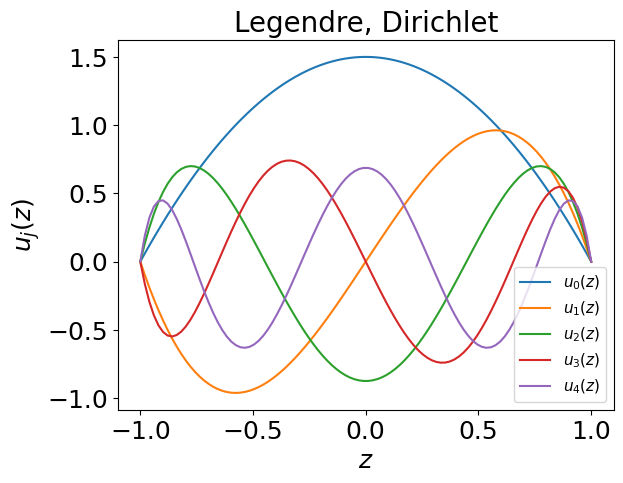
\includegraphics[width=0.7\textwidth]{figures/legendre-dirichlet.png}
	\caption{Compact Legendre combinations satisfying Dirichlet boundary condition.}
	\label{fig:legendre-dirichlet}
\end{figure}
The necessary parameters to make $u_k(\pm 1) = 0$ are $a_k=0, b_k=-1$. The basis functions are therefore,
\begin{equation}
	u_k(z) = L_k(z) - L_{k+2}(z).
\end{equation}
The first 5 basis functions are shown in Fig.~\ref{fig:legendre-dirichlet}.

\subsubsection*{Fixed-Open Boundary}
\begin{figure} [htbp]
	\centering
	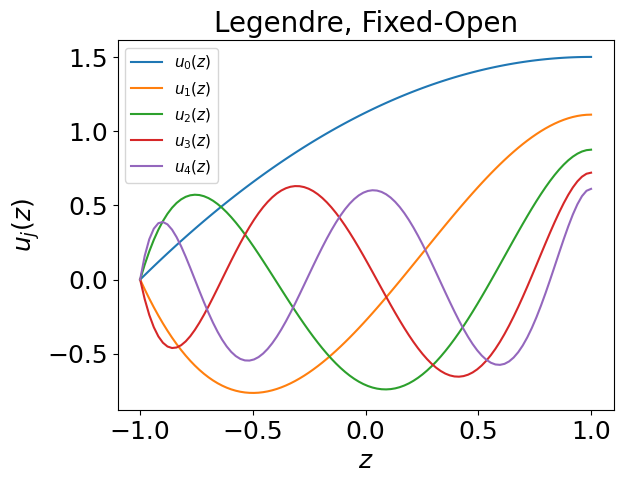
\includegraphics[width=0.7\textwidth]{figures/legendre-fixed-open.png}
	\caption{Compact Legendre combinations satisfying fixed-open boundary condition.}
	\label{fig:legendre-fixed-open}
\end{figure}
The necessary parameters to make $u_k(-1)=u_k'(1)=0$ are $a_k=(2k+3)/(k+2)^2, b_k=-(k+1)^2/(k+2)^2$. The basis functions are therefore,
\begin{equation}
	u_k(z) = L_k(z) + \frac{2k+3}{(k+2)^2}L_{k+1}(z) - \frac{(k+1)^2}{(k+2)^2}L_{k+2}(z)
\end{equation}
The first 5 basis functions are shown in Fig.~\ref{fig:legendre-fixed-open}.

By setting $\tilde{v}(z) = \sum_{j=0}^{N} c_ku_k(z)$, $\tilde{v}$ satisfies the boundary conditions automatically. There is no need to modify the matrices in Eq.~(\ref{eq:pep-matrix-equation}).

To evaluate the matrix elements, inner products are calculated by numerical integration, in this thesis Simpson's rule is used. Eq.~(\ref{eq:operator-matrix-M}) and Eq.~(\ref{eq:operator-matrix-N}) become

\begin{align}
	M_{jk} & = 2i \sum_{m}^{M} w_m \Delta z_m \left[\psi_{j}\left(v_0\pdv{}{z} +\pdv{v_0}{z} \right)u_{k}\right]_{z_m} \\
	N_{jk} & = \sum_{m}^{M} w_m \Delta z_m \left\{
	\psi_{j} \left[(1-v_0^2)\pdv[2]{}{z} -\left(3v_0 + \frac{1}{v_0}\right)\pdv{v_0}{z}\pdv{}{z}
		- \left(1-\frac{1}{v_0^2}\right)\left(\pdv{v_0}{z}\right)^2 - \left(v_0+\frac{1}{v_0}\right)\pdv[2]{v_0}{z}\right] u_{k} \right\}_{z_m},
\end{align}
where $M$ is the number of points, $\Delta z_m = 2/M$, and $w_m$ are coefficients corresponding to the quadrature rule employed. In this case,
\begin{equation}
	w_n = \begin{cases}
		1/3, \text{if $m=0,M$}    \\
		4/3, \text{if $m$ is odd} \\
		2/3, \text{if $m\neq 0,M$ and $m$ is even}.
	\end{cases}
\end{equation}

After solving Eq.~(\ref{eq:pep-matrix-equation}), the eigenvector $\mathbf{c}$ can be used to reconstruct the eigenfunctions. See Listing.~\ref{code:spectral-galerkin} for more details.

\begin{lstlisting}[language=Python, float, floatplacement=H, caption={Pseudocode for solving polynomial eigenvalue problem using Lengendre-Galerkin method}, label=code:spectral-galerkin]
import numpy as np
from scipy.special import lengendre # lengendre polynomials
from scipy.integrate import simpson # simpson quadrature
# collocation points, differentiation matrices
N = 25 # number of basis functions
M = 101 # number of points
x, D1, D2 = Chebyshev(M, "symmetric", "CH")
# use this basis for drichlet boundary
u = lambda x,k: (legendre(k) + (2*k+3)/(k+2)**2*legendre(k+1) - (k+1)**2/(k+2)**2*legendre(k+2))(x)
# use this basis for fixed-open boundary
u = lambda x,k: (legendre(k) - legendre(k+2))(x)
# solve polynomial eigenvalue problem
A11 = np.zeros_like(D1)
A12 = np.eye(*D1.shape)
A21 = np.zeros((N,N),dtype=complex)
A22 = np.zeros((N,N),dtype=complex)
for i in range(N):
    for j in range(N):
		A21[i,j] = simpson(
			- u(x,i)*(1-v0**2)*(D2@u(x,j))
			+ u(x,i)*(3*v0+1/v0)*(D1@v0)*(D1@u(x,j))
			+ u(x,i)*(1-1/v0**2)*(D1@v0)**2*u(x,j) 
			+ u(x,i)*(v0+1/v0)*(D2@v0)*u(x,j),
			x=x)
		A22[i,j] = -2j*simpson(u(x,i)*v0*(D1@u(x,j)) + u(x,i)*(D1@v0)*u(x,j),x=x)
A = np.block([[A11, A12],
              [A21, A22]])
omega, C = np.linalg.eig(A)
# construct eigenfunctions
V = np.zeros((x.size, C.shape[1]),dtype=complex)
for i in range(C.shape[1]):
    for k in range(N):
        V[:, i] += C[k,i]*u(x, k)
\end{lstlisting}


\section{Spectral Theory in Finite-Dimensional Normed Spaces}
Spectral method transforms the polynomial eigenvalue problem to an algebraic eigenvalue problem. For completion, some important linear algebra results are included in this section.

Let $X$ be a finite dimensional normed space and $\hat{T}: X \to X$ a linear operator. Since any linear operator can be represented by a matrix, the spectral theory of $\hat{T}$ is essentially matrix eigenvalue theory \cite{kreyszig_introductory_1978}. Let $A$ be a matrix representation of $\hat{T}$, then we have the definition.

\begin{definition} [Kryszig \cite{kreyszig_introductory_1978}]
	An eigenvalue of a square matrix $A$ is a complex number $\lambda$ such that
	\[ Ax = \lambda x \]
	has a solution $x\neq 0$.This $x$ is called an \textbf{eigenvector} of $A$ corresponding to that eigenvalue $\lambda$.The set $\sigma(A)$ of all eigenvalues of $A$ is called the \textbf{spectrum} of $A$. Its complement $\rho(A) = \mathbb{C}-\sigma(A)$ in the complex plane is called the \textbf{resolvent} set of $A$.
\end{definition}

By choosing different bases in $X$, we can have different matrix representation of $\hat{T}$. We need to make sure the eigenvalues of a linear operator is independent of the basis chosen. Fortunately, a theorem ensures that.

\begin{theorem} [Kryszig \cite{kreyszig_introductory_1978}]
	All matrices representing a given linear operator $\hat{T}: X \to X$ on a finite dimensional normed space $X$ relative to various bases for $X$ have the same eigenvalues.
\end{theorem}


Moreover, we don't need to worry about the existence of eigenvalues of a linear operator. The following theorem shows the existence of them.
\begin{theorem} [Kryszig \cite{kreyszig_introductory_1978}]
	A linear operator on a finite dimensional complex normed space $X\neq{O}$ has at least one eigenvalue.
\end{theorem}

\section{Spectral Pollution and Spurious Modes}
In this section, we will discuss an important phenomenon we observe throughout the numerical experiments using spectral method. It is the phenomenon of spectral pollution. Then we will provide a method to filter these spurious modes.

Spectral pollution refers to the phenomenon which some eigenvalues are not converging to the correct value when the mesh density is increased. The wrong eigenvalues are referred as spurious modes. When solving eigenvalue problems using spectral methods with finite difference or finite element approximations, spectral pollution might occur \cite{llobet_spectral_1990}. The cause of the spectral pollution is originated from the improper discretization of the differential operators. In the following sections, we are going to take a closer look at the differential operators in finite difference method, and reveal the occurrence of spurious modes when solving Eq.~(\ref{eq:constant-v-problem}) with supersonic velocity profile.

\subsection{Analysis of Numerical Spectrum} \label{sec:analysis-of-numerical-spectrum}
In this section, we will analyze the analytical and numerical dispersion relation of the following problem,
\[
	\omega^2\tilde{v} + 2i\omega v_0\pdv{\tilde{v}}{z} + (1-v_0^2)\pdv[2]{\tilde{v}}{z} = 0, \quad v(\pm 1) = 0
\]

It is a special case, i.e. $v_0=$constant, of a more general problem Eq.~(\ref{eq:polynomial-eigenvalue-problem}). The analytical dispersion relation can be obtained by substituting $\tilde{v} = \exp(-i\omega t + kx)$ into the above equation,
\begin{equation} \label{dispersion-relation}
	\omega = k(v_0 \pm 1).
\end{equation}
The dispersion relation suggests that the eigenvalue $\omega$ should be real.

Now let's analyze the dispersion relation produced by finite difference. To do this we need to first understand the effect of the differential operators on function $\tilde{v}$ in finite difference. If we assume $\tilde{v}\sim \exp(ikx)$, and let $\beta\equiv kh/2$. Then in finite difference discretization scheme, the differential operators $\dv*[n]{z}$ are equivalent to the following factors \cite{llobet_spectral_1990},
\begin{equation}
	\begin{aligned}
		\dv[0]{z} \quad \to \quad & G_0 = 1                                                               \\
		\dv[1]{z} \quad \to \quad & G_1 = [\exp(2i\beta)-\exp(-2i\beta)]/2h = (i/h)\sin(2\beta)           \\
		\dv[2]{z} \quad \to \quad & G_2 = [\exp(2i\beta)-2-\exp(-2i\beta)]/h^2 = (2/h^2)(\cos(2\beta)-1).
	\end{aligned}
	\label{eq:G-operator}
\end{equation}

Using the G-operators, Eq.~(\ref{eq:G-operator}), the discretized equation of Eq.~(\ref{eq:constant-v-problem}) becomes
\begin{equation} \label{eq:discretized-eq-G}
	(\omega^2G_0 + \omega G_1 + G_2)\tilde{v} = 0.
\end{equation}

Solving Eq.~(\ref{eq:discretized-eq-G}), we obtain the numerical dispersion relation,
\begin{equation}
	\omega = \frac{2\sin(\beta)}{h}\left(v_0 \pm \sqrt{1 - v_0^2\sin[2](\beta)}\right).
	\label{eq:dispersion-relation-G}
\end{equation}

Given $h$ (fixed the mesh resolution), we see that
\begin{itemize}
	\item $\omega$ is real for all $k$ if $v_0 < 1$.
	\item $\omega$ is complex for large $k$, more specifically $k>h/2\arcsin(1/v_0)$, if $v_0 > 1$.
	\item For small $k$, meaning $k\to 0$, Eq.~(\ref{eq:dispersion-relation-G}) is a good representation for the analytical dispersion relation, Eq.~(\ref{dispersion-relation}).
\end{itemize}

\begin{figure}[htbp!]
	\centering
	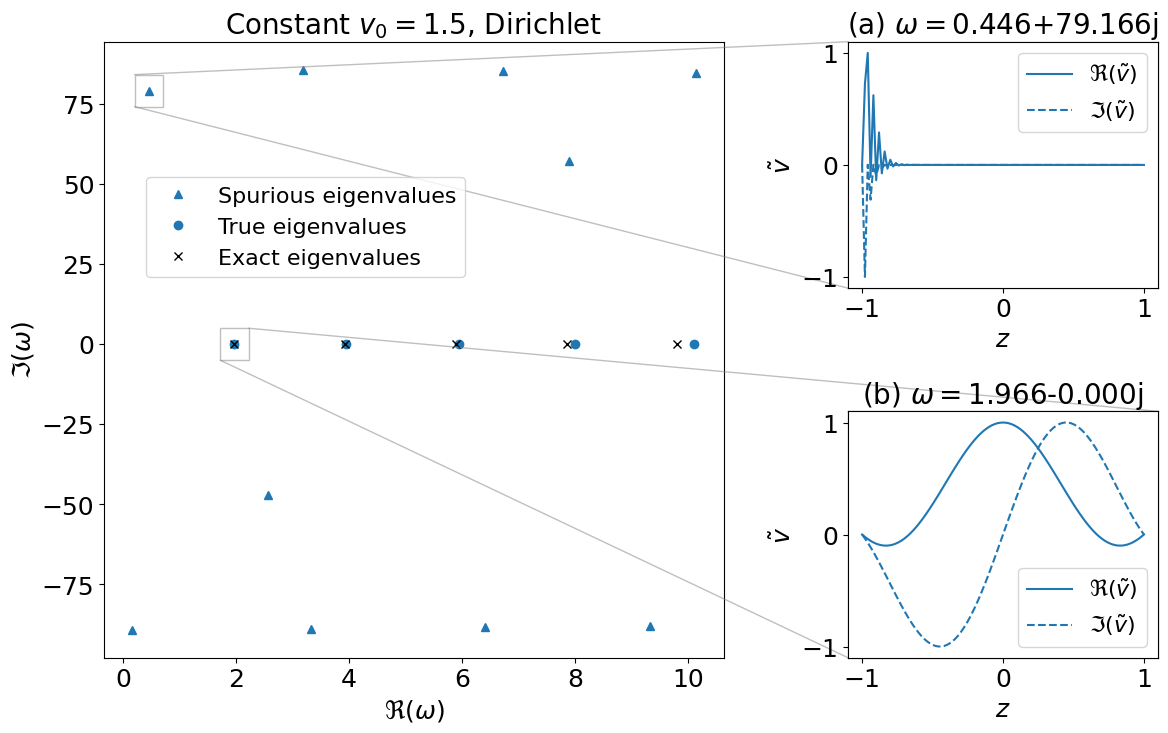
\includegraphics[width=\textwidth]{figures/eigenmodes-FD.png}
	\caption{(a) Eigenfunction corresponding to a spurious eigenvalue, the eigenfunction has weird shape. (b) Eigenfunction corresponding to a true eigenvalue.}
	\label{fig:eigenmodes-FD}
\end{figure}

In this simple case of solving Eq.~(\ref{eq:discretized-eq-G}), one way to filter the spurious modes is to remove modes with high-oscillation. That is removing modes with wave number $k>h/2 \arcsin(1/v_0)$. However, this is not possible in general cases because Eq.~(\ref{eq:dispersion-relation-G}) is only valid if finite-difference is used, and it requires the exact solution to the discretized problem Eq.~(\ref{eq:discretized-eq-G}) which is not available for non-constant velocity profile.

\subsection{Convergence Test}
To filter the spurious modes is by doing a "convergence test". Since the frequency Eq.~(\ref{eq:dispersion-relation-G}) is changing with mesh resolution $h$. From Fig.~\ref{fig:convergence-test} we see that only the true eigenmodes converge while the eigenvalues of spurious eigenmodes changes dramatically under different resolutions. By simply solving the discretized problem using spectral method under different mesh resolution, we can pick up the true eigenmodes by observing their convergence, and filter out the spurious eigenmodes which change dramatically with varying resolution.

\begin{figure} [htbp]
	\centering
	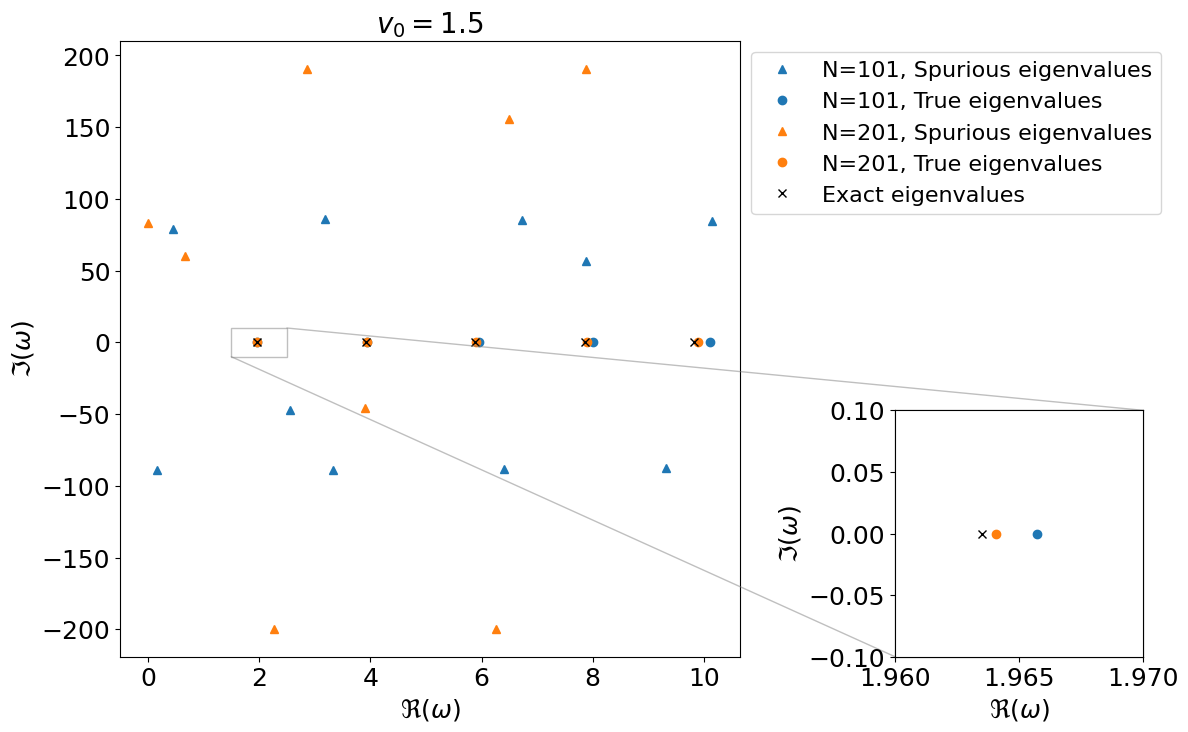
\includegraphics[width=\textwidth]{figures/convergence-test.png}
	\caption{The figure shows eigenvalues under different resolutions. True eigenvalues converge to the analytical eigenvalues as resolution increases. Spurious eigenvalues diverges with no obvious pattern.}
	\label{fig:convergence-test}
\end{figure}

\section{Plasma Flow with Constant Velocity Profile}
In this section, we will compute the eigenmodes of the constant velocity problem, Eq.~(\ref{eq:constant-v-problem}), with Dirichlet boundaries and the same problem with fixed-open boundaries, using spectral methods. More specifically, spectral-collocation and spectral-Galerkin methods will be employed. Then spurious modes will be filtered using the convergence test prescribed in previous section. Since we have already derived the exact solutions for the constant velocity cases in Sec.~\ref{sec:analytical-solutions}, we can ensure the accuracy and reliability of the numerical methods by comparing the numerical results to the analytical ones. The parameters of spectral methods are summarized in Table.~(\ref{table:parameters}). For spectral-collocation method, we use 101 points, and for spectral-Galerkin method we use 101 points and 30 basis functions.

\begin{table} [htbp]
	\centering
	\caption{With Dirichlet boundary condition, all methods have good accuracy, so using 101 nodes in the region $[0,1]$ is enough. For FE and SE methods, we use 50 basis functions.}
	\begin{tabular}{|c|c|c|}
		\hline
		                              & Collocation & Galerkin \\
		\hline
		M (number of points)          & 101         & 101      \\
		\hline
		N (number of basis functions) &             & 30       \\
		\hline
	\end{tabular}
	\label{table:parameters}
\end{table}

\subsection{Constant Subsonic Velocity Case}
Eq.~(\ref{eq:constant-v-problem}) is a special case of a more general polynomial eigenvalue problem Eq.~(\ref{eq:polynomial-eigenvalue-problem}). The existence of the exact solution allows us to verify the correctness of each method's implementation. This also serves as a reference to the accuracy spectral methods can achieve.

In summary, the plasma flow constant subsonic velocity profile is stable in the magnetic nozzle under both boundary conditions, Dirichlet boundary and fixed-open boundary. If the velocity is supersonic, then the plasma flow is stable is the boundary is Dirichlet, and is unstable if the boundary is fixed-open.

\subsubsection*{Dirichlet Boundary}
\begin{table} [htpb!]
	\centering
	\caption{Relative errors of first five eigenvalues obtained by spectral methods in constant subsonic velocity case with Dirichlet boundary condition. Numerical results agree with exact solution well.}
	\begin{tabular}{|c|c|c|c|c|c|}
		\hline
		$v_0=0.5$   & $\omega_1$     & $\omega_2$     & $\omega_3$     & $\omega_4$     & $\omega_5$     \\
		\hline
		Collocation & 3.48944421e-14 & 6.72512513e-14 & 1.59603736e-14 & 9.81718764e-15 & 4.07098462e-15 \\
		\hline
		Galerkin    & 4.09596742e-14 & 1.65697986e-14 & 4.97650778e-14 & 3.27344763e-13 & 4.11444935e-12 \\
		\hline
	\end{tabular}
	\label{table:eigenvalue-error-constant-subsonic-dirichlet}
\end{table}

\begin{figure}[htpb!]
	\centering
	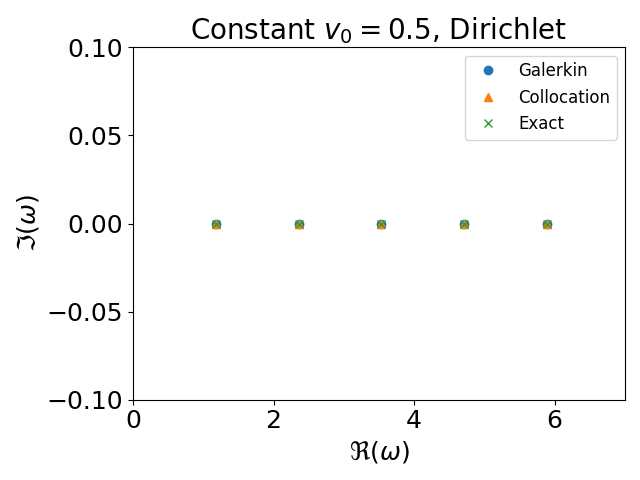
\includegraphics[width=0.7\linewidth]{figures/constant-subsonic-dirichlet.png}
	\caption{Showing the first five eigenvalues obtained by spectral-collocation and spectral-Galerkin methods. The plasma flow in the magnetic nozzle with constant subsonic velocity and Dirichlet boundary is stable. Spectral methods agree with exact eigenvalues.}
	\label{fig:constant-subsonic-dirichlet}
\end{figure}

Fig.~\ref{fig:constant-subsonic-dirichlet} shows that the eigenvalues obtained by spectral methods agree with the theoretical eigenvalues. Table.~\ref{table:eigenvalue-error-constant-subsonic-dirichlet} shows us the relative error $\abs{\omega_{numeric} - \omega_{analytic}}/\abs{\omega_{analytic}}$ is about $10^{-14}$ for each eigenvalue. Spectral methods indeed have high accuracy. Since the eigenvalues have almost zero imaginary parts, we consider the plasma flow with constant subsonic velocity in the magnetic nozzle with Dirichlet boundary is stable.


\subsubsection*{Fixed-Open Boundary}
\begin{table} [htbp!]
	\centering
	\caption{Relative error of each eigenvalue. Notice that the mode index starts from 0. These results agree with theory.}
	\begin{tabular}{|c|c|c|c|c|c|}
		\hline
		$v_0=0.5$   & $\omega_0$     & $\omega_1$     & $\omega_2$     & $\omega_3$     & $\omega_4$     \\
		\hline
		Collocation & 2.36006260e-12 & 1.95269435e-13 & 6.78183927e-14 & 2.43078107e-14 & 4.17011610e-14 \\
		\hline
		Galerkin    & 2.52491323e-12 & 2.19414097e-13 & 1.82417919e-13 & 5.92948284e-13 & 4.41481039e-12 \\
		\hline
	\end{tabular}
	\label{table:eigenvalue-error-fixed-open-subsonic}
\end{table}

\begin{figure}[htbp!]
	\centering
	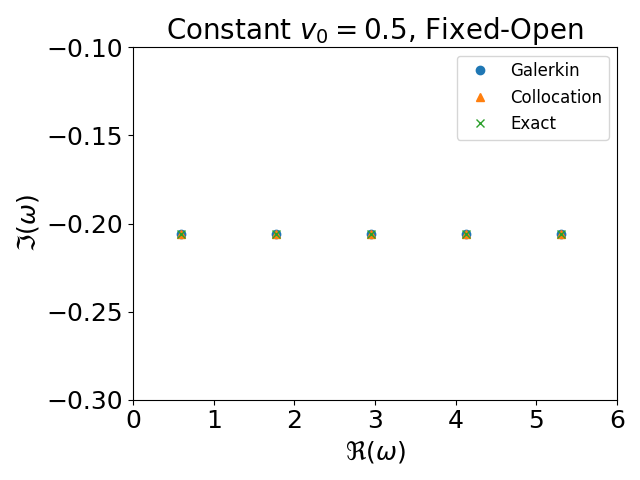
\includegraphics[width=0.7\linewidth]{figures/constant-subsonic-fixed-open.png}
	\caption{Showing the first five eigenvalues obtained by spectral-collocation and spectral-Galerkin methods. The plasma flow in the magnetic nozzle with constant subsonic velocity and fixed-open boundary is stable. Spectral methods agree with exact eigenvalues.}
	\label{fig:constant-subsonic-fixed-open}
\end{figure}

As shown in Fig.~\ref{fig:constant-subsonic-fixed-open} and Table.~\ref{table:eigenvalue-error-fixed-open-subsonic}, the numerical eigenvalues obtained by the spectral methods agree with the analytical eigenvalues. The relative errors $\abs{\omega_{numeric} -\omega_{analytic}}/\abs{\omega_{analytic}}$ are about $10^{-13}$. Again both spectral methods show good accuracy. Because the eigenvalues have negative imaginary parts, meaning the perturbations will exponential decay, so the plasma flow with constant subsonic velocity in the magnetic nozzle with fixed-open boundary is stable.

\subsection{Constant Supersonic Velocity Case}
In supersonic case, as predicted by Sec.~\ref{sec:analysis-of-numerical-spectrum}, spurious modes occur. Convergence test was used to filter the spurious modes.

\subsubsection*{Dirichlet Boundary}
\begin{table} [htbp!]
	\centering
	\caption{Relative error of first five filtered eigenvalues obtained by spectral methods in constant subsonic case under Dirichlet boundary. Numerical results agree with the theory, but we see the accuracy of eigenvalues obtained from spectral-Galerkin method drops after the 3rd one.}
	\begin{tabular}{|c|c|c|c|c|c|}
		\hline
		$v_0=1.5$   & $\omega_1$     & $\omega_2$     & $\omega_3$     & $\omega_4$     & $\omega_5$     \\
		\hline
		Collocation & 2.08984845e-13 & 9.29501612e-14 & 4.24537846e-14 & 3.38103217e-14 & 1.74476052e-14 \\
		\hline
		Galerkin    & 1.64805562e-13 & 6.09485884e-14 & 6.81795167e-12 & 1.95656738e-09 & 1.54134402e-07 \\
		\hline
	\end{tabular}
	\label{table:eigenvalue-error-dirichlet-supersonic}
\end{table}

\begin{figure}[htbp!]
	\centering
	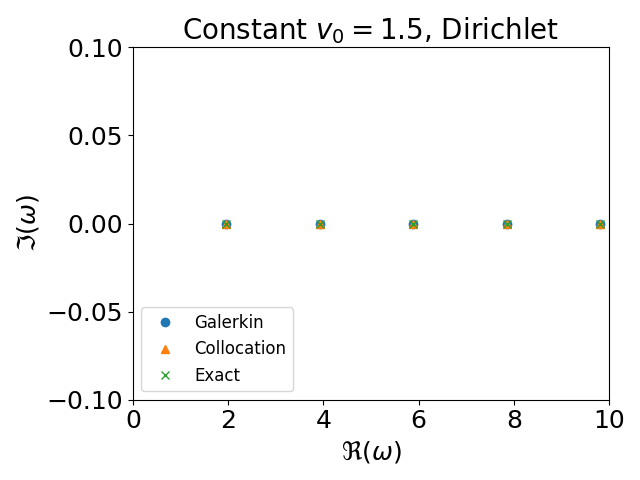
\includegraphics[width=0.7\linewidth]{figures/constant-supersonic-dirichlet.png}
	\caption{Showing the first five true eigenvalues obtained by spectral-collocation and spectral-Galerkin methods. The plasma flow in the magnetic nozzle with constant supersonic velocity and Dirichlet boundary is stable. Spectral methods agree with exact eigenvalues.}
	\label{fig:constant-supersonic-dirichlet}
\end{figure}

The first five filtered eigenvalues obtained by the two spectral methods are shown in Fig.~\ref{fig:constant-subsonic-dirichlet} and Table.~\ref{table:eigenvalue-error-dirichlet-supersonic} shows us the relative error of each of them compare to the corresponding exact eigenvalues. Good agreement between the spectral methods and the theoretical eigenvalues is shown. However, we see that the accuracy of spectral-Galerkin method drops for larger eigenvalues. The plasma flow with constant supersonic velocity is stable in the magnetic nozzle with Dirichlet boundary.

\subsubsection*{Fixed-Open Boundary}
\begin{table} [htbp!]
	\centering
	\caption{Relative error of first five eigenvalues obtained by spectral methods in constant supersonic case under fixed-open boundary. Results agree with theory. The accuracy of spectral-Galerkin method drops after first few eigenvalues.}
	\begin{tabular}{|c|c|c|c|c|c|}
		\hline
		$v_0=1.5$   & $\omega_0$     & $\omega_1$     & $\omega_2$     & $\omega_3$     & $\omega_4$     \\
		\hline
		Collocation & 5.10516649e-11 & 3.58709292e-12 & 8.72529437e-13 & 3.24263319e-13 & 1.34297439e-13 \\
		\hline
		Galerkin    & 5.38682371e-11 & 4.31902441e-12 & 1.44799870e-12 & 8.02395621e-11 & 2.05280524e-09 \\
		\hline
	\end{tabular}
	\label{table:eigenvalue-error-fixed-open-supersonic}
\end{table}

\begin{figure}[htbp!]
	\centering
	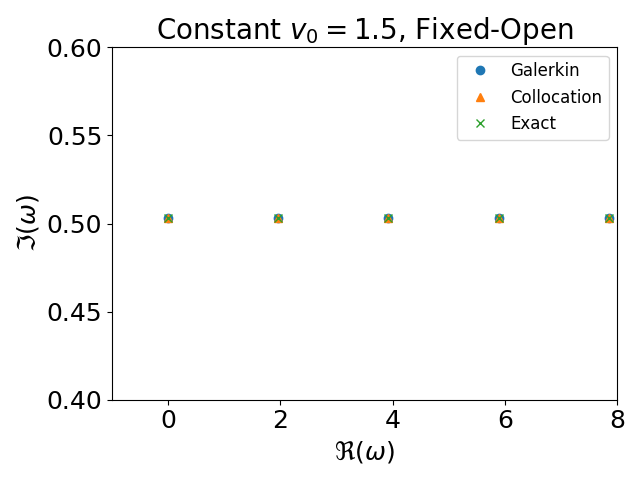
\includegraphics[width=0.7\linewidth]{figures/constant-supersonic-fixed-open.png}
	\caption{Showing the first five true eigenvalues obtained by spectral-collocation and spectral-Galerkin methods. The plasma flow in the magnetic nozzle with constant supersonic velocity and fixed-open boundary is unstable.}
	\label{fig:constant-supersonic-fixed-open}
\end{figure}

Table.~\ref{table:eigenvalue-error-fixed-open-supersonic} shows relative error for the first five filtered eigenvalues obtained by different spectral methods. We see that the accuracy of spectral-Galerkin method drops for larger eigenvalues. Fig.~\ref{fig:constant-supersonic-fixed-open} shows us that plasma flow with constant supersonic velocity is unstable in the magnetic nozzle with fixed-open boundary.

\section{Plasma Flow with Spatial Varying Velocity Profiles}
In previous section we have already verify the accuracy of spectral methods by comparing the numerical results to the analytical solutions to the eigenvalue problem with constant velocity plasma flow, Eq.~(\ref{eq:constant-v-problem}). In this section we will apply spectral methods to the eigenvalue problem with spatial varying velocity profiles. That is Eq.~(\ref{eq:polynomial-eigenvalue-problem}) with Dirichlet boundary and fixed-open boundary conditions. The parameters for spectral methods are the same as Table.~\ref{table:parameters}.

\subsection{Subsonic Case}
In this case, the plasma flows with subsonic velocity. The velocity profile is spatial varying and will reach its maximum $0.5$ Mach at the nozzle throat $z=0$. The velocity profile is the orange line shown in Fig.~\ref{fig:velocity-profiles}. When applying spectral methods, no spurious modes were found in subsonic case. Similar to the case with constant velocity profile, we experiment with two boundary conditions: Dirichlet boundary and fixed-open boundary. We found that the plasma flow is stable when the boundary condition is Dirichlet and is stable (except ground mode) when using fixed-open boundary.

\subsubsection*{Dirichlet Boundary}
\begin{figure} [htbp!]
	\centering
	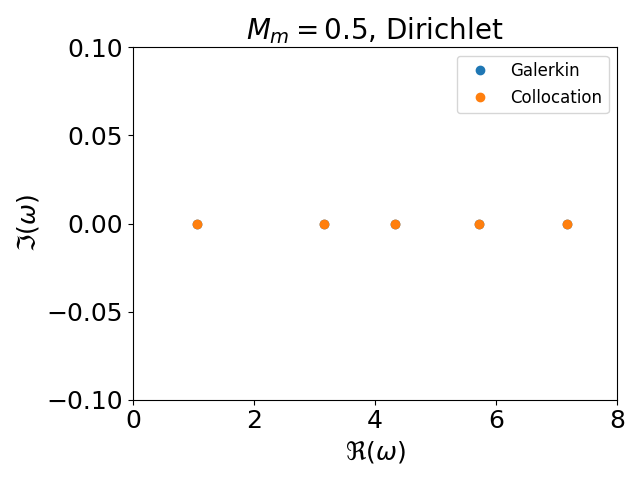
\includegraphics[width=0.7\linewidth]{figures/subsonic-drichlet.png}
	\caption{Showing the first five eigenvalues obtained by spectral-collocation and spectral-Galerkin method. This indicates that the subsonic plasma flow in magnetic nozzle with Dirichlet boundary is stable. Two methods agree with each other well enough the eigenvalues are overlapped.}
	\label{fig:subsonic-dirichlet}
\end{figure}
With Dirichlet boundary condition, $\tilde{v}(\pm 1) =0$, the subsonic plasma flow in magnetic nozzle is stable. Fig.~\ref{fig:subsonic-dirichlet} shows the first five eigenvalues obtained by different spectral methods. The two methods, spectral-collocation and spectral-Galerkin, agree with each other well enough so the eigenvalues are overlapped on the figure. These eigenvalues has zero imaginary parts (to be more specific, $\abs{\Im{\omega}} < 10^{-13}$), meaning that the subsonic plasma flow in the magnetic nozzle is stable.

\subsubsection*{Fixed-Open Boundary}
\begin{figure} [htbp!]
	\centering
	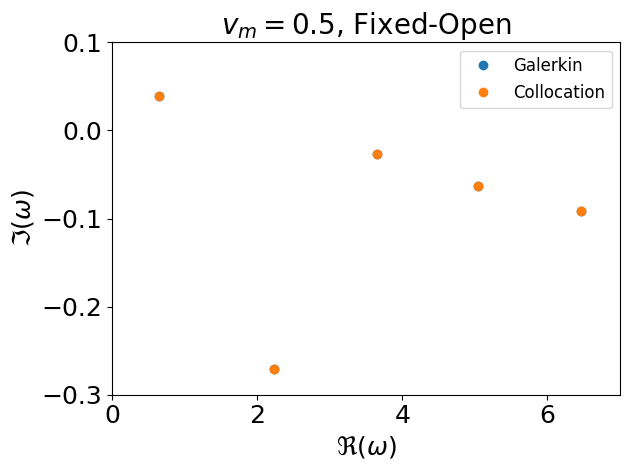
\includegraphics[width=0.7\linewidth]{figures/subsonic-fixed-open.png}
	\caption{Showing the first five eigenvalues obtained by spectral-collocation and spectral-Galerkin method. This indicates that the subsonic plasma flow in magnetic nozzle with fixed-open boundary is stable (except ground mode). Two methods agree with each other well enough the eigenvalues are overlapped.}
	\label{fig:subsonic-fixed-open}
\end{figure}
Fig.~\ref{fig:subsonic-fixed-open} shows the first five eigenvalues obtained by the two spectral methods. The results agree with each other well enough so the eigenvalues are overlapped. We see that the eigenvalues have negative imaginary parts (except ground mode), indicating that the subsonic plasma flow in the nozzle with fixed-open boundary is stable (except ground mode).

\subsection{Supersonic Case}
In this subsection, we are going to investigate the instability of supersonic plasma flow in the magnetic nozzle. The velocity profile is the purple line shown in Fig.~\ref{fig:velocity-profiles}. The plasma flow reaches its minimum velocity $1.5$ Mach at the nozzle throat $z=0$. When applying spectral methods, spurious modes occur and we need to apply convergence test to extract the true eigenvalues. We found that the supersonic plasma flow is stable when the Dirichlet boundary condition was used, and is unstable the boundary is fixed-open.

\subsubsection*{Dirichlet Boundary}
\begin{figure} [htbp!]
	\centering
	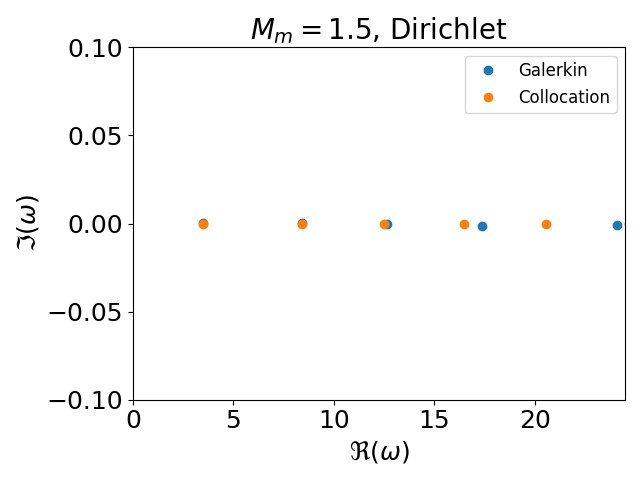
\includegraphics[width=0.7\linewidth]{figures/supersonic-drichlet.png}
	\caption{Showing the first five true eigenvalues obtained by spectral-collocation and spectral-Galerkin method. This indicates that the supersonic plasma flow in magnetic nozzle with Dirichlet boundary is stable. Two methods agree well on the first 3 eigenmodes, and starts to deviate from each other after that. Nevertheless, these eigenvalues have near-zero imaginary parts. The eigenvalues obtained by spectral-Galerkin have imaginary parts within $\pm10^{-3}$ and the eigenvalues obtained by spectral-collocation have imaginary parts within $\pm10^{-13}$.}
	\label{fig:supersonic-dirichlet}
\end{figure}
As shown Fig.~\ref{fig:supersonic-dirichlet}, the two spectral methods agree well on the first three eigenvalues but starts to have noticeable difference afterward. Despite having different real parts in the eigenvalues, these eigenvalues all have near-zero imaginary parts. The imaginary parts of the eigenvalues obtained by spectral-collocation method are within $\pm10^{-13}$, and the imaginary parts of the eigenvalues obtained by spectral-Galerkin method are within $\pm10^{-3}$. This suggests the supersonic plasma flow in the magnetic nozzle with Dirichlet boundary is stable.

\subsubsection*{Fixed-Open Boundary}
\begin{figure} [htbp!]
	\centering
	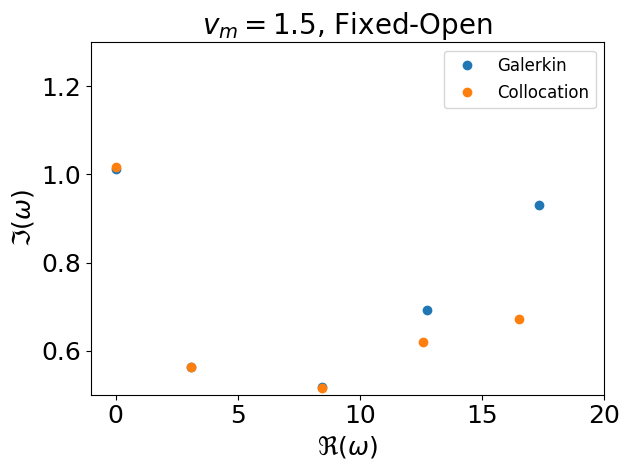
\includegraphics[width=0.7\linewidth]{figures/supersonic-fixed-open.png}
	\caption{Showing the first five true eigenvalues obtained by spectral-collocation and spectral-Galerkin method. Two methods agree well on the first three modes, and start to have significant difference after that. Despite having some different eigenvalues, these eigenvalues all have positive imaginary parts, suggesting that the supersonic plasma flow in the magnetic nozzle with fixed-open boundary is unstable.}
	\label{fig:supersonic-fixed-open}
\end{figure}
In Fig.~\ref{fig:supersonic-fixed-open}, we see that the two spectral methods agree well on the first three eigenvalues but starts to have noticeable difference afterward. Despite having different eigenvalues after the third eigenvalue, these eigenvalues all have positive imaginary parts, suggesting the supersonic plasma flow in the magnetic nozzle with fixed-open boundary is unstable.
